% INTRODUCCIÓN

\cleardoublepage

\chapter{Introducción}
\label{introduccion}

Cuando pensamos en drones, estamos pensando en dispositivos que podemos pilotar con un \textit{smartphone} y que nos permiten realizar videos y fotos a vista de pájaro. Lo que no siempre se tiene en cuenta es la capacidad de estos dispositivos para poder ejecutar algoritmos complejos, como son por el ejemplo aquellos que permiten al dispositivo hacer el seguimiento de un objeto a través de la cámara a tiempo real. Esto es lo que se conoce como \textit{object tracking} y es el punto fundamental de nuestro trabajo.
\medskip


Recientes algoritmos y estudios alrededor del \textit{object tracking}, entre ellos \citet{activetracking} o \citet{zhou2021space}, se centran fundamentalmente en el reconocimiento del objeto y en la posición de éste con respecto a las coordenadas X e Y en relación al centro de la imagen a través de la cámara incorporada para guiar las acciones del dispositivo. Es lo que se conoce como \textit{passive tracking}. Este tipo de algoritmos han ganado más atención debido a la simplicidad del problema y los avances en reconocimiento de objetos. Lo cual los hace idóneos para una aplicación industrial.
\medskip

Otros intentos de realizar \textit{object tracking} con aprendizaje supervisado se realizan utilizando modelos en simuladores tanto del dron como de las personas. Sin embargo, la idea del presente trabajo es la aplicación de diferentes técnicas de inteligencia artificial para lograr un agente que sea capaz de realizar el seguimiento utilizando simplemente imágenes que provengan del propio dispositivo en el cual se desplegará el agente.
\medskip

Sin embargo, el objetivo en nuestro caso es poder realizar el seguimiento a tiempo real de una persona a través de la cámara del dispositivo utilizando para ello visión por computador y técnicas de aprendizaje por refuerzo para controlar las acciones a tomar en cada momento. Lo que se conoce como \textit{active tracking}. 
\medskip

\begin{figure}[ht!]
\centering
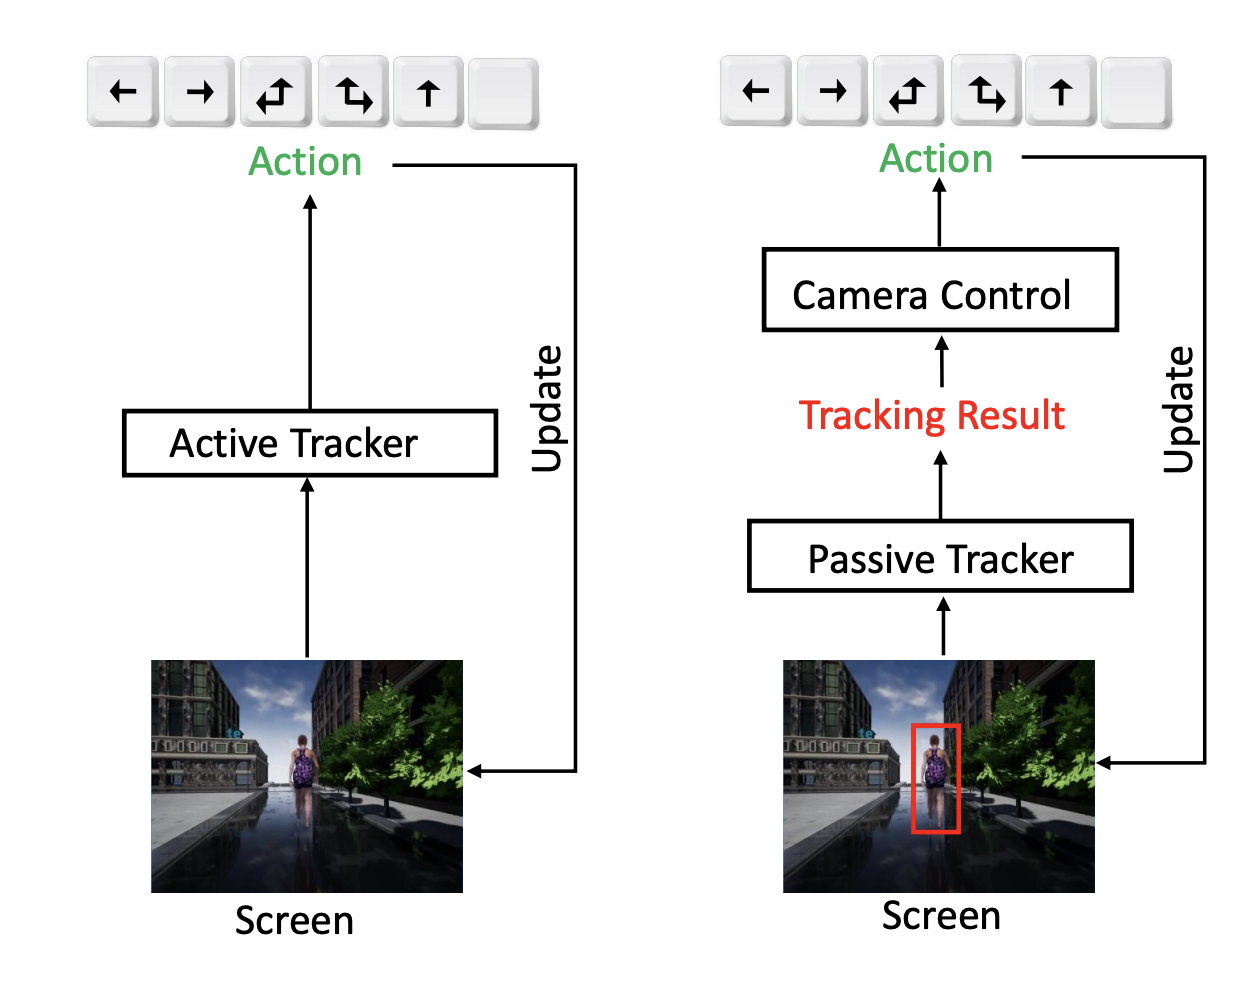
\includegraphics[scale=0.4]{figuras/active_tracking_vs_passive_tracking.png}
\caption[A la izquierda, el pipeline utilizado durante active tracking. A la derecha, el pipeline utilizado en passive tracking.]{A la izquierda, el pipeline utilizado durante active tracking. A la derecha, el pipeline utilizado en passive tracking. Imagen tomada de \citet{luo2019end}.}
\label{fig-active-tracking}
\end{figure}
\medskip

Para ello, no solo utilizaremos técnicas de aprendizaje por refuerzo, sino también técnicas de aprendizaje supervisado (redes convolucionales para el reconocimiento de objetos) sobre imágenes, para la obtención de nuestro conjunto de datos inicial, tal y como explicaremos en las siguientes secciones.
\medskip

El desarrollo del proyecto se llevará a cabo utilizando lenguaje Python y la librería \href{https://pytorch.org/}{PyTorch} para el desarrollo de los modelos. El código completo estará disponible para su visualización en un repositorio de \href{https://github.com/lucaswerner90/msc-degree-ai}{GitHub}, a excepción de los pesos de los diferentes agentes que se vayan guardando durante el entrenamiento debido al tamaño individual de cada uno de estos archivos y a las imágenes que se fueron registrando durante el entrenamiento.


\section{Acotación del problema}
\label{acotacion-del-problema}

Debido a que nos movemos en un entorno real en el cual las posibilidades tanto de actuación sobre el entorno como de error son muy amplias, no solo debido a la aleatoriedad del mismo sino también al número de acciones que podemos tomar, debemos definir ciertas restricciones que nos permitan abordar el problema de una manera más sencilla.
\medskip

En primer lugar, nos centraremos en obtener una solución que sea viable en entornos en los cuales las condiciones externas no sean un impedimento para el buen funcionamiento de nuestro algoritmo. Esto quiere decir que durante el desarrollo y testeo de los algoritmos obviamos factores tales como el viento, las condiciones de humedad o el grado de iluminación en un momento dado, que pudiesen afectar al rendimiento del dispositivo.
\medskip

Por otro lado, debido a que el espacio de acciones disponibles es muy alto, en una primera fase dispondremos de tan solo 3: 

\begin{itemize}
  \item Girar a la derecha.
  \item Girar a la izquierda.
  \item Mantenerse en el mismo lugar.
\end{itemize}
\medskip

Tanto el giro a la derecha como el giro a la izquierda se realizará en el dispositivo de manera controlada, esto quiere decir que nos moveremos siempre utilizando el mismo ángulo de giro. 
\medskip

Si quisiéramos añadir además un ángulo de giro variable junto con la acción a tomar podríamos hacerlo como parte de la salida de nuestro algoritmo, aunque involucraría un entrenamiento más prolongado en el tiempo, lo cual es un factor importante tal y como detallaremos más adelante.
\medskip

Teniendo en cuenta este espacio inicial de acciones, la evaluación de los diferentes agentes será valorada positiva o negativamente con respecto al eje X exclusivamente. Esto quiere decir que consideraremos que el algoritmo funciona de forma correcta si es capaz de moverse de tal manera que la persona se encuentre siempre centrada en el eje horizontal y no en el eje vertical.
\medskip

En cuanto a la detección de la persona, tenemos en cuenta que nuestro dispositivo solo realizará el seguimiento de una sola persona, debido a la complejidad que esto supondría en cuanto al funcionamiento de nuestro algoritmo. Obviamos un escenario real y plausible que es el de encontrarnos en una misma imagen con múltiples personas, en cuyo caso deberíamos también de desarrollar un mecanismo de selección de la persona a la cual quisiéramos seguir.
\medskip

Por lo tanto, quedándonos con una parte simplificada del problema, podemos centrarnos en conseguir un algoritmo que pueda considerarse como el mínimo viable para conseguir nuestro objetivo.
\medskip

\section{Dispositivo utilizado}
\label{dispositivo-utilizado}

Para el desarrollo del proyecto se utilizará el dispositivo \href{https://store.dji.com/de/shop/tello-series}{DJI Tello}, ya que nos proporciona una interfaz de programación compatible con nuestras necesidades: control del dispositivo y transmisión de datos a través de una API en lenguaje Python.
\medskip


\begin{figure}[ht!]
  \centering
  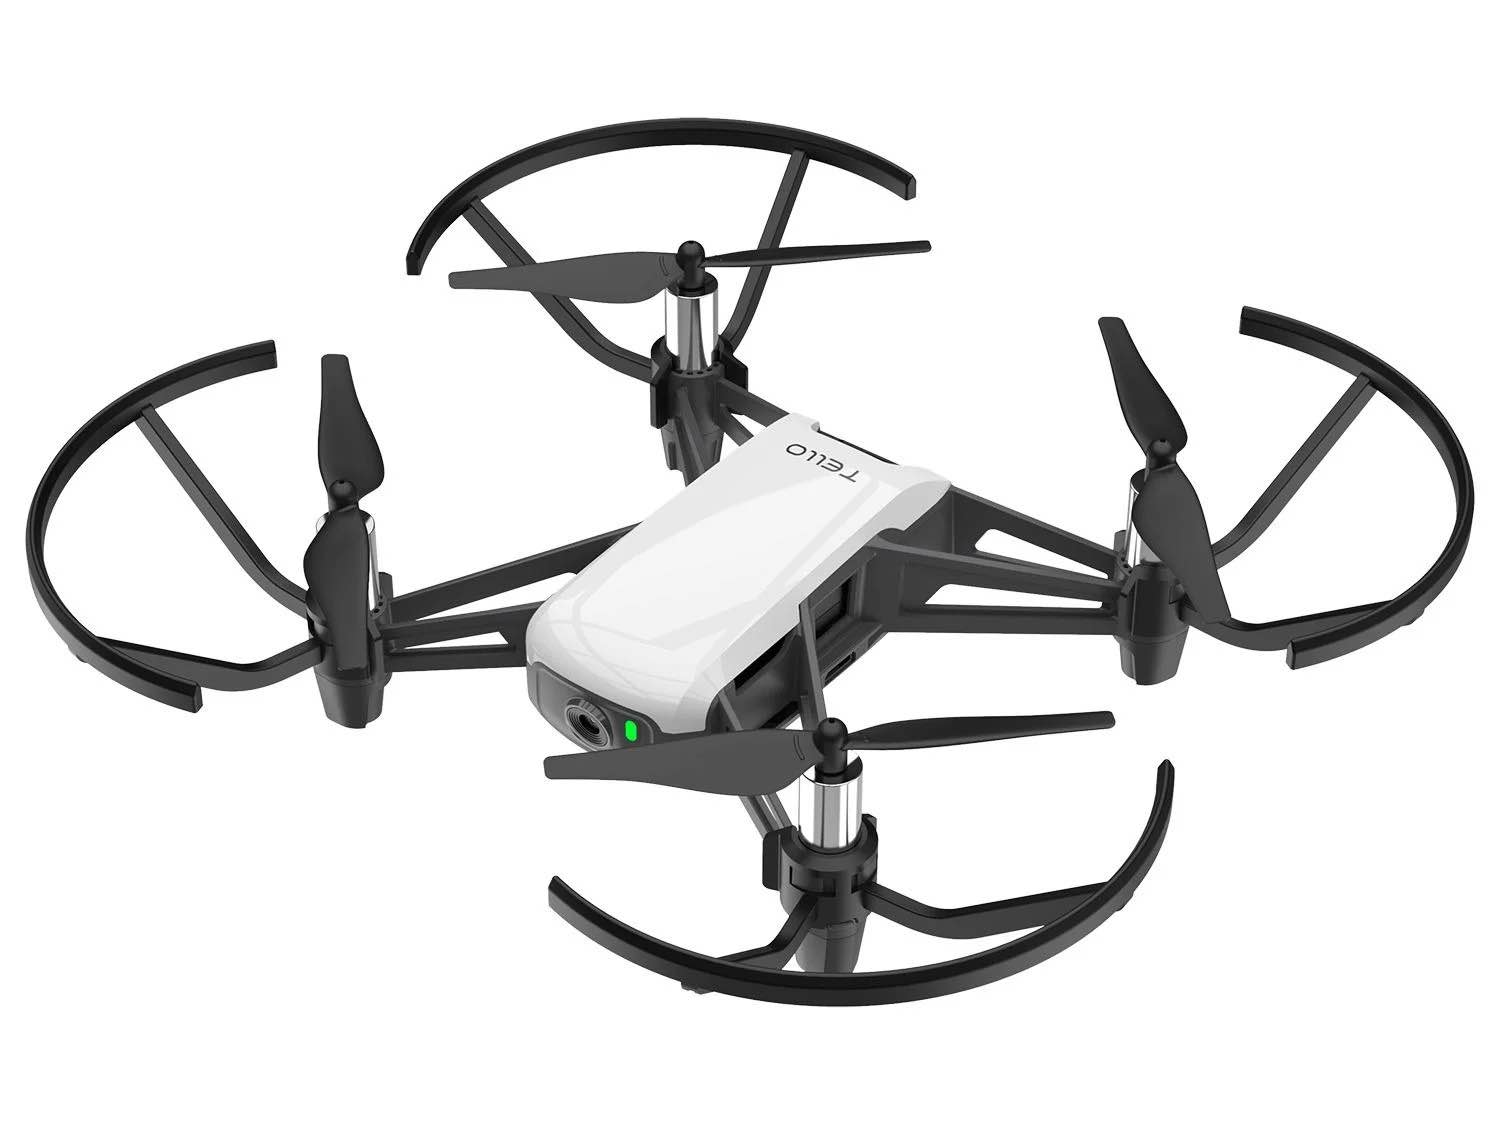
\includegraphics[scale=0.2]{figuras/dispositivo_utilizado.png}
  % \caption[Así aparece el rótulo en el índice]{Así aparece el rótulo en el texto.}
  \caption[DJI Tello. Dispositivo utilizado durante el proyecto]{Imagen del dispositivo utilizado durante el proyecto.}
  \label{fig-dron}
\end{figure}


El dispositivo cuenta con una cámara integrada con una resolución máxima de 1280x720 píxeles, la cual creemos que es suficiente para el desarrollo del trabajo.
\medskip

Un punto negativo del uso de drones como dispositivo de captura es el poco rendimiento de las baterías durante el vuelo. Concretamente, el dron utilizado permanece en vuelo unos 13 minutos como máximo. Por este motivo es importante mencionar que el entrenamiento no se realizará directamente en el dron, sino que se usará en una fase inicial y final del proyecto para evaluar a los agentes una vez que estos estén entrenados.
\medskip

Además, durante el desarrollo inicial del proyecto se pudo observar una latencia reseñable al intentar comunicar el dispositivo con el ordenador a la hora de transmitir las imágenes y de poder enviar señales de control debido a la débil conexión WiFi entre ambos puntos de comunicación. El intentar solucionar este problema no solo consumió tiempo de ejecución del proyecto sino que también nos impide poder llevar a cabo pruebas de control más realistas y nos acotará el margen de ejecución de nuestras pruebas finales.
\medskip

\section{Marco teórico}

En esta sección haremos una breve introducción a los diferentes componentes teóricos que nos iremos encontrando a lo largo del trabajo. Empezaremos repasando los principales conceptos relacionados con el aprendizaje por refuerzo y en qué se diferencia de otros tipos de entrenamiento. 
\medskip

Después haremos una introducción a cada uno de los algoritmos que vamos a utilizar y comentaremos brevemente las diferencias y el por qué los elegimos.
Por último comentaremos los \textit{Transformers}\citep{transformers} y en especial los \textit{Vision Transformers}\citep{visiontransformers}, ya que serán utilizados durante uno de los experimentos que explicaremos en la sección \ref{experimentacion} .
\medskip

\subsection{Aprendizaje por refuerzo}
\label{aprendizaje-por-refuerzo}

\textit{"La idea de que nosotros aprendemos a través de la interacción con nuestro entorno es probablemente lo primero que se nos ocurre cuando pensamos en la naturaleza del aprendizaje"}, \citep{sutton2018reinforcement}.
\medskip

\begin{figure}[H]
  \centering
  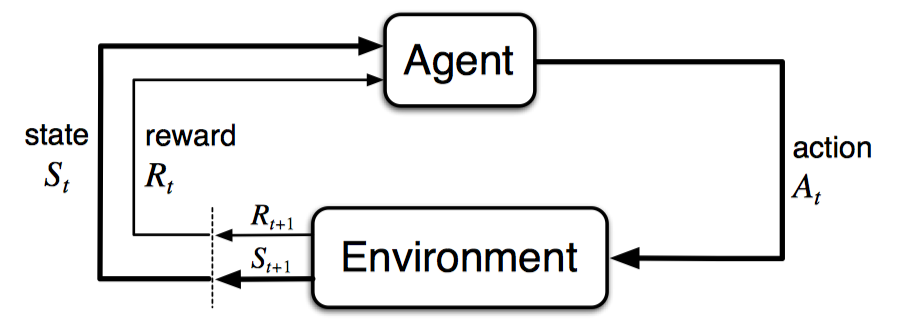
\includegraphics[width=1\textwidth]{figuras/RL_diagram.png}
  % \caption[Así aparece el rótulo en el índice]{Así aparece el rótulo en el texto.}
  \caption[Componentes del aprendizaje por refuerzo y la interacción entre ellos.]{Componentes del aprendizaje por refuerzo y la interacción entre ellos.}
  \label{fig-reinforcement-learning-components}
\end{figure}

Podemos decir que el aprendizaje por refuerzo es la formalización de la idea anterior, en concreto, es la rama de la inteligencia artificial cuyo principio se basa en la interacción de un agente con un entorno a través de lo que llamamos acciones. Dichas acciones obtienen una recompensa que el agente recibe y en base a estas recompensas, se refuerzan las acciones positivas y se penalizan las negativas, es decir, el objetivo del agente es maximizar las recompensas obtenidas a lo largo del tiempo.
\medskip

Durante los últimos años se pudo ver cómo está rama fue cobrando más importancia por casos exitosos como el de \textit{AlphaGo} \citep{silver2016mastering}, creado por la empresa \href{deepmind.com}{DeepMind}, que derrotó al campeón mundial en el juego Go, un hito que era considerado como extraordinario debido al número de combinaciones por movimiento que el juego contiene.
\medskip

\begin{figure}[ht!]
  \centering
  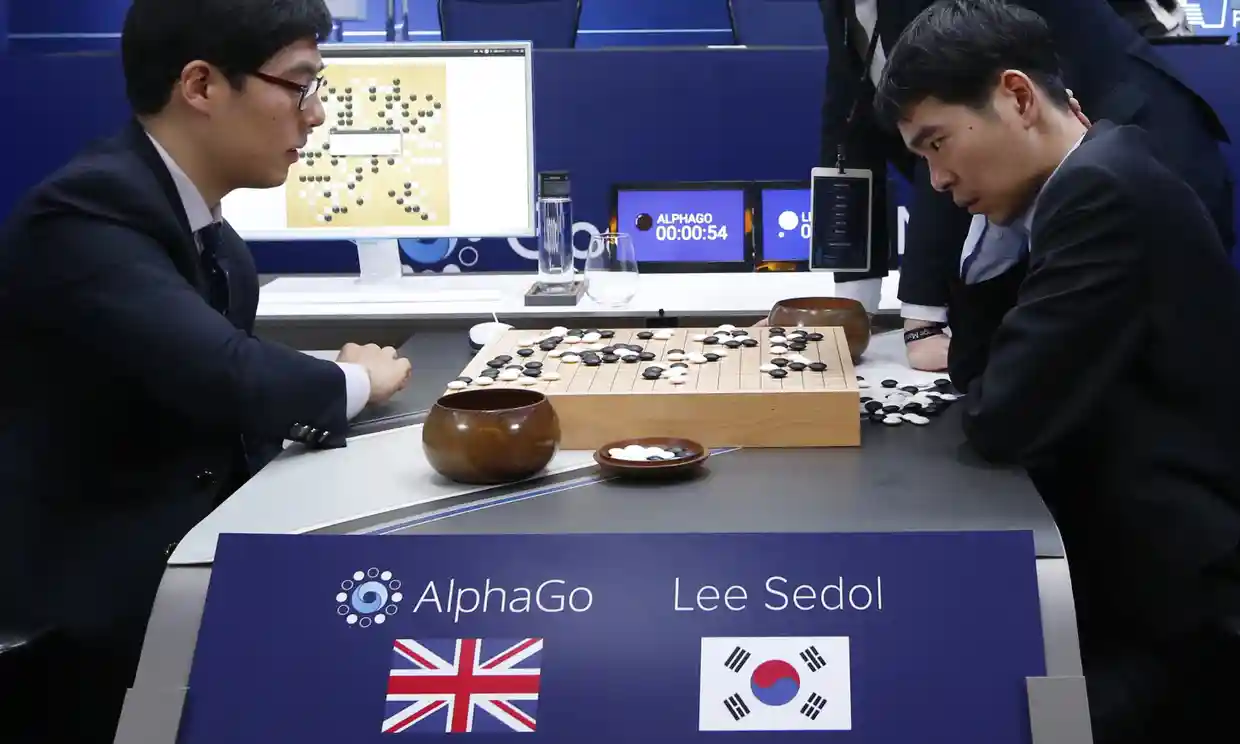
\includegraphics[width=1\textwidth]{figuras/alphago.png}
  % \caption[Así aparece el rótulo en el índice]{Así aparece el rótulo en el texto.}
  \caption[Imagen tomada durante una de las partidas entre \textit{AlphaGO} y Lee Sedol.]{Imagen tomada durante una de las partidas entre \textit{AlphaGO} y Lee Sedol. Fuente: \href{https://www.theguardian.com/technology/2016/mar/15/alphago-what-does-google-advanced-software-go-next}{The Guardian}.}
  \label{fig-alphago}
\end{figure}

Aunque se suele asociar al aprendizaje por refuerzo con aplicaciones como \textit{AlphaGo}, o el aún más reciente caso de \textit{AlphaStar} \citep{alphastar}, gracias a los avances tanto en algoritmos como en el campo del \textit{deep learning}, vemos que con más frecuencia nos encontramos con ejemplos reales en el uso de estas técnicas, lo cual nos anima a realizar nuestro trabajo sobre ellas.
\medskip

\subsection{Algoritmos \textit{Policy Gradient}}
\label{algoritmo-policy-gradient}

El subgrupo de algoritmos \textit{Policy Gradient} \citep{sutton1999policy} se basan en la optimización de la política de elección de acciones del agente, es decir, producen politicas de acción estocásticas. Esto contrasta con el subgrupo de algoritmos \textit{Q-Learning} \citep{mnih2013playing} que se basan en la optimización de la función de valor y que producen políticas deterministas.
\medskip

Una ventaja de estos algoritmos es que por lo general son más estables y confiables que los basados en \textit{Q-Learning} y que pueden actuar sobre espacio de acciones continuos (aunque finalmente nosotros nos centraremos en un espacio discreto). Es por ello que serán nuestro foco durante la ejecución del proyecto.
\medskip


\begin{figure}[ht!]
  \centering
  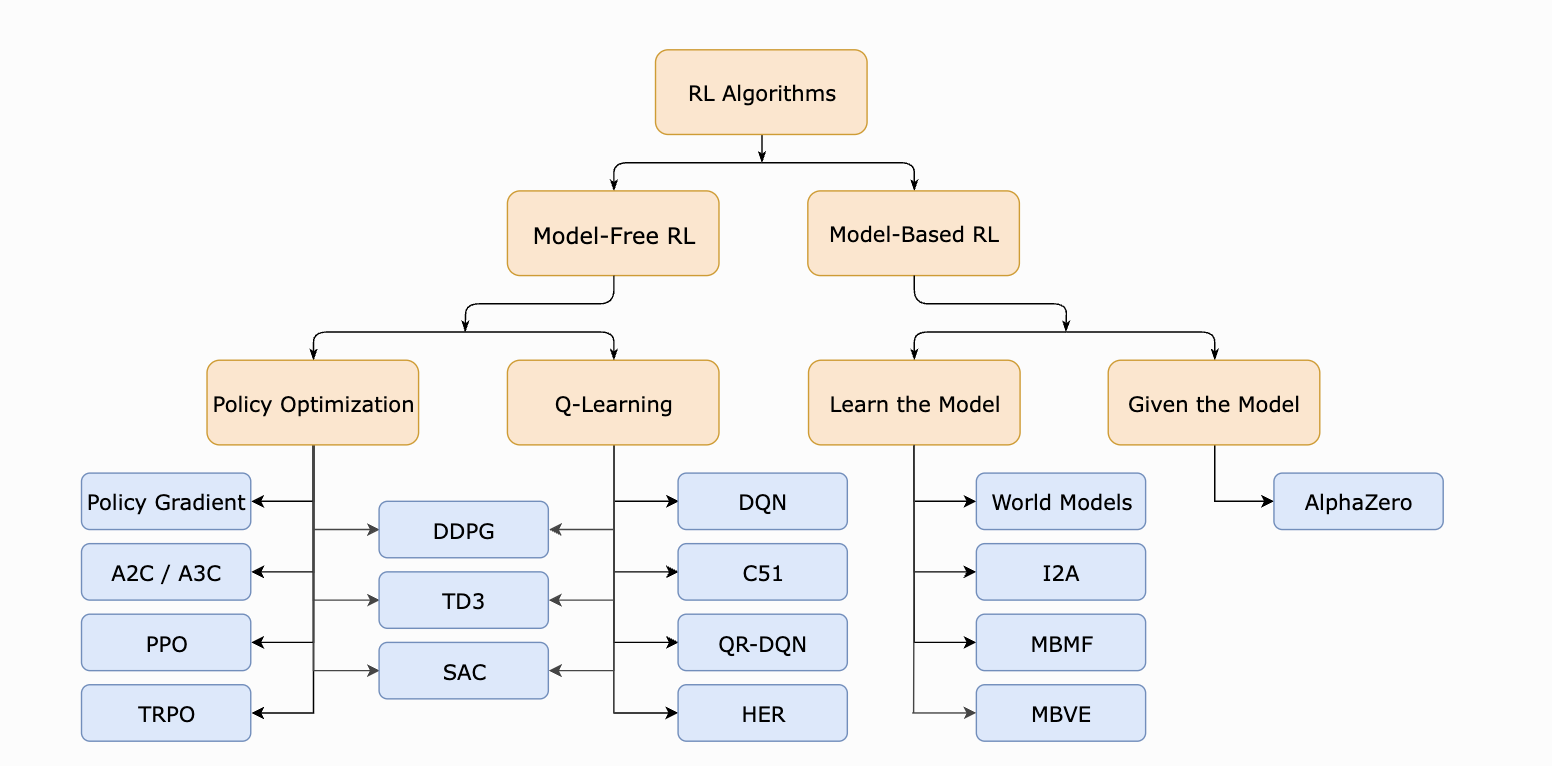
\includegraphics[width=1\textwidth]{figuras/rl_algorithms_classification.png}
  % \caption[Así aparece el rótulo en el índice]{Así aparece el rótulo en el texto.}
  \caption[Categorización de algoritmos de aprendizaje por refuerzo.]{Categorización de algoritmos de aprendizaje por refuerzo. Fuente: \href{https://spinningup.openai.com/en/latest/spinningup/rl_intro2.html}{OpenAI}.}
  \label{fig-rl-algorithms-family}
\end{figure}

\subsection{Algoritmo Actor-Critic}
\label{algoritmo-actor-critic}

Siguiendo con la misma familia de algoritmos, la diferencia en este caso es que el agente tiene que aprender no solamente qué acción tomar en cada observación del estado sino que también aprende a calcular cuál es la recompensa estimada a futuro. Para lo cual, necesitamos dos redes neuronales. La parte responsable de calcular la acción recomendada se llama \textit{actor}, mientras que aquella que se encarga de decirnos la recompensa futura se llama \textit{critic}.
\medskip

Una forma sencilla de entenderlo sería verlo como que nuestra parte \textit{actor} nos dice qué hacer, mientras que la red \textit{critic} nos indica cuánto de bien lo estamos haciendo.
\medskip

\begin{figure}[ht!]
  \centering
  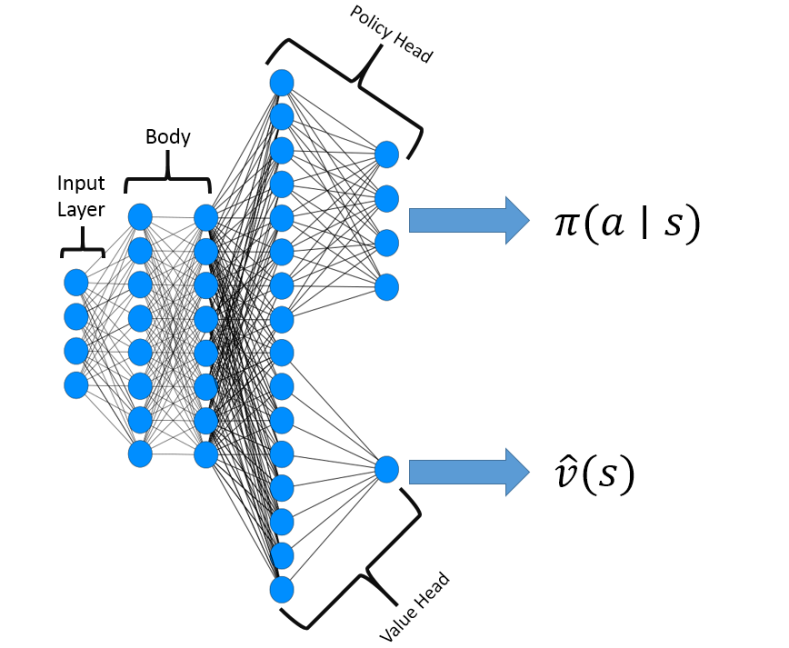
\includegraphics[width=.5\textwidth]{figuras/actor_critic_arquitecture.png}
  % \caption[Así aparece el rótulo en el índice]{Así aparece el rótulo en el texto.}
  \caption[Visualización de una red \textit{Actor Critic}.]{Visualización de una red \textit{Actor Critic}. Fuente: \href{https://www.datahubbs.com/two-headed-a2c-network-in-pytorch/}{DataHubbs}.}
  \label{fig-actor-critic-arquitecture}
\end{figure}

\subsection{Transformers y Vision Transformers}
\label{vision-transformers}

Sin entrar en muchos detalles en cuanto a cómo funcionan los \textit{Transformers} y los \textit{Vision Transformers}, haremos un breve repaso de las características unicas de estas redes, ya que uno de los experimentos nombrados en la sección \ref{resultados-actor-critic-vision-transformers} será el de un agente con una red de tipo \textit{Vision Transformer} \citep{visiontransformers}, que se encargará de realizar la transformación de la imagen de entrada.
\medskip

\begin{figure}[H]
  \centering
  \subfloat[Arquitectura \textit{Transformer} original]{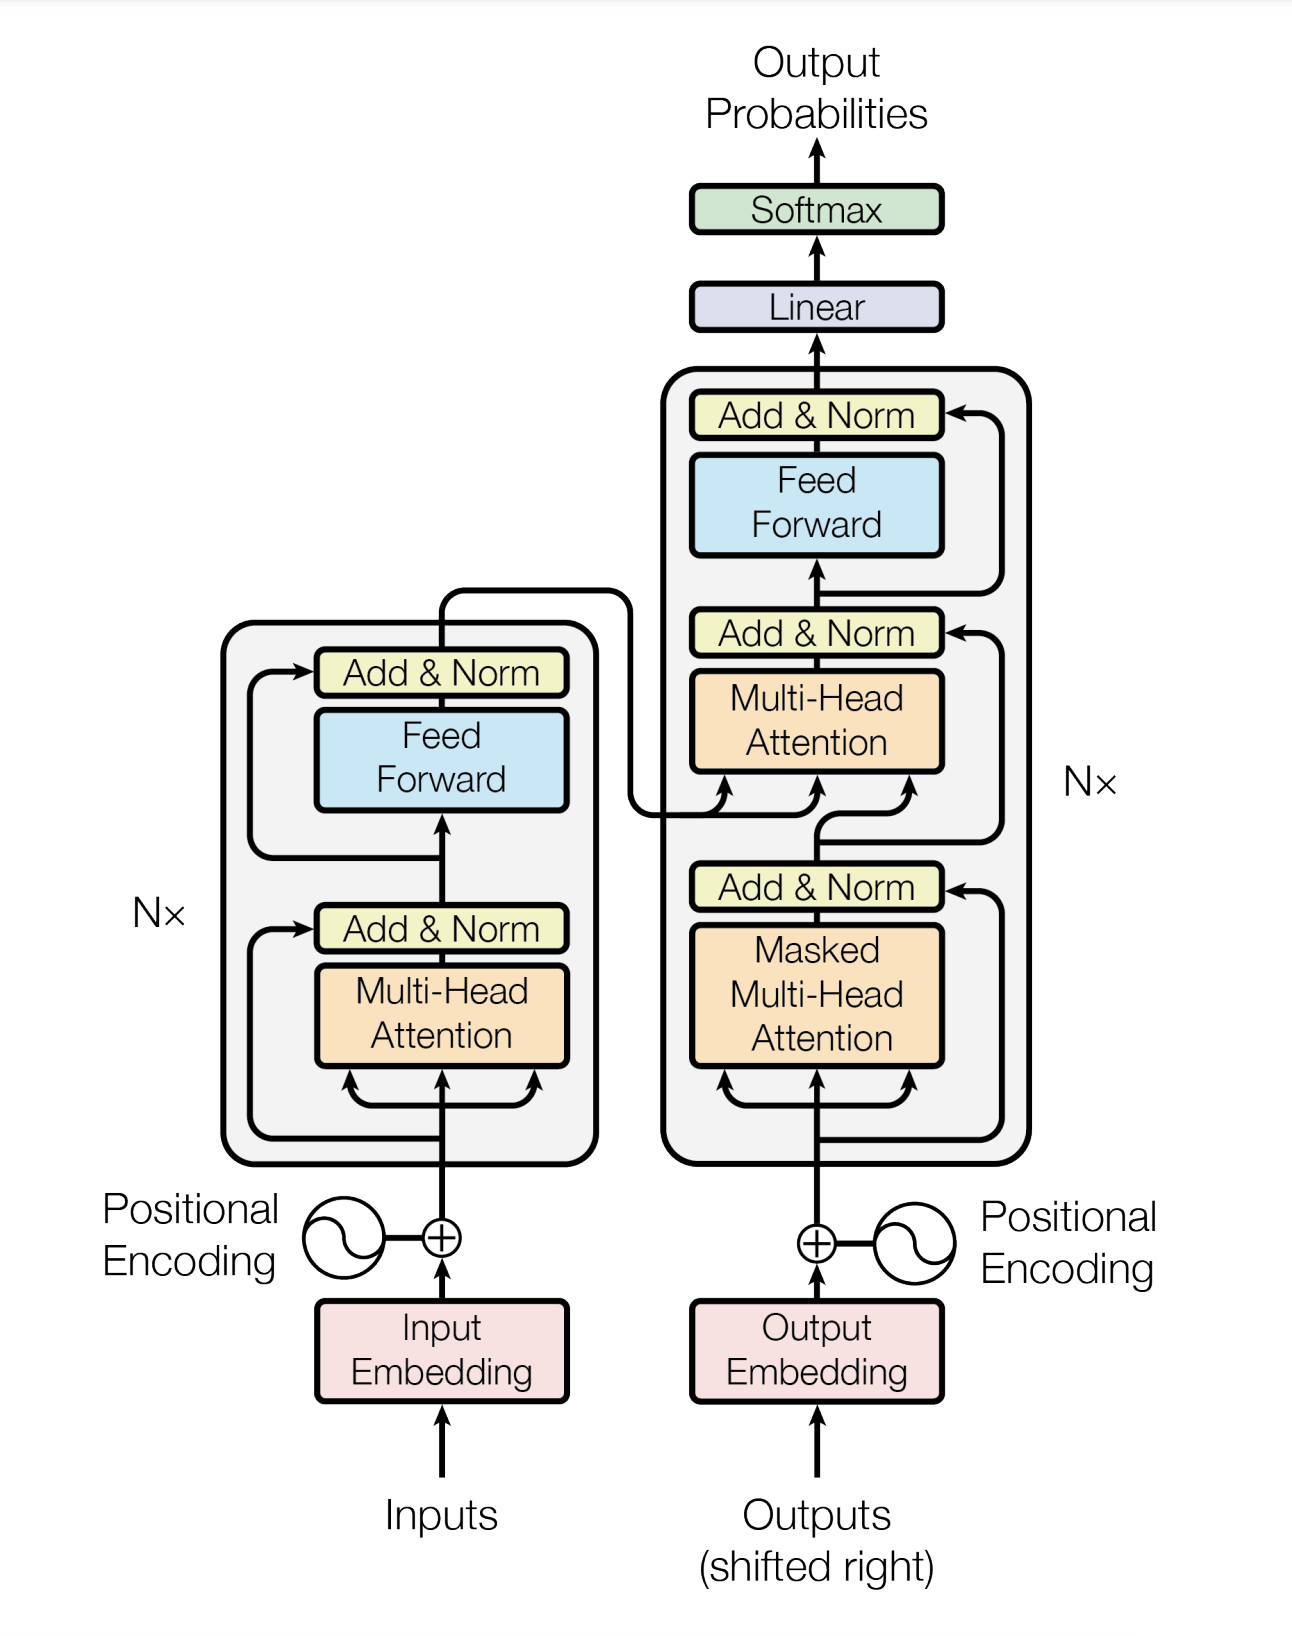
\includegraphics[scale = 0.2]{figuras/transformer_architecture.png}}
  \subfloat[Arquitectura propuesta para \textit{Vision Transformers}]{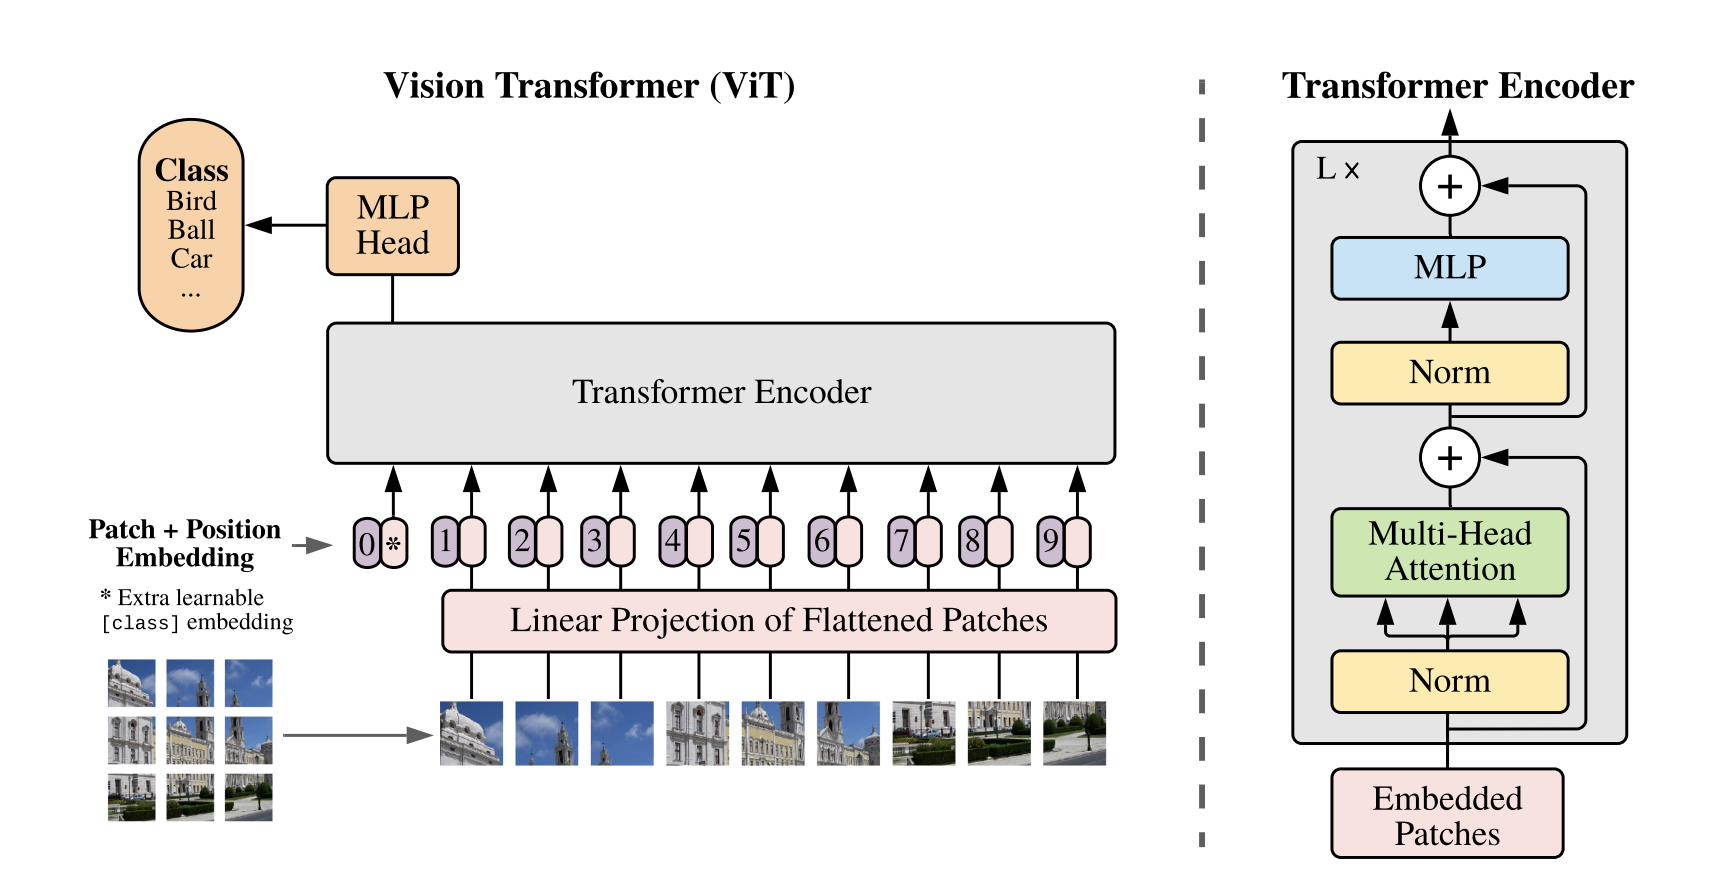
\includegraphics[scale = 0.3]{figuras/vision_transformers.png}} 
  % \caption[Así aparece el rótulo en el índice]{Así aparece el rótulo en el texto.}
  \caption[Imágenes de las arquitecturas (a) \textit{Transformer} y (b) \textit{Vision Transformer}]{Imágenes de las arquitecturas (a) \textit{Transformer} y (b) \textit{Vision Transformer}}
  \label{fig-vision-transformer}
\end{figure}

Las redes basadas en \textit{Attention}, en particular las redes \textit{Transformers}, desarrolladas inicialmente por Google, se han convertido en la elección por defecto en problemas de lenguaje natural o \glossary{NLP}, ya que gracias a su eficiencia computacional y su escalabilidad, es posible entrenar modelos de más de 100 billones de parámetros. La idea detrás de estas redes es solucionar los problemas que presentan las redes neuronales recurrentes o \glossary{RNN}, tales como las redes \glossary{LSTM} o \glossary{GRU}, las cuales no son capaces de captar dependencias a largo plazo, tal y como podemos encontrarnos en un texto de una novela.
\medskip

Aunque los \textit{Transformers} son ampliamente utilizados en procesamiento de lenguaje natural, las arquitecturas de redes convolucionales o \glossary{CNN} seguian siendo el tipo de red dominante en el campo de la visión por computador. Es por ello que, inspirados en la arquitectura original de \textit{Transformer} y en el éxito que estas contaban (y aún cuentan), se buscó aplicar los mismos principios en la visión por computador. Esto es lo que dio lugar a los \textit{Vision Transformer}, cuya idea principal es la de partir una imagen en segmentos o \textit{patches} y ser capaces de aplicar capas de Attention a cada uno de ellos. 
\medskip

A día de hoy nos encontramos muchas versiones disponibles y preentrenadas. Durante la ejecución de nuestro experimento utilizaremos un modelo disponible en la web \href{https://huggingface.co/docs/transformers/model_doc/vit#transformers.ViTModel}{HuggingFace}.
\medskip

En concreto utilizamos un modelo entrenado por Google, cuya entrada es una imagen de 224x224 píxeles, que será luego dividida en 16 parches de 14x14 píxeles y que fue entrenada en el conjunto de datos \textit{ImageNet21k} \citep{imagenet21k}.
\medskip

La salida de este modelo, es decir, la entrada a nuestro agente será un vector de tamaño 197x512, donde la primera dimensión representa el tamaño de la secuencia en la cual nuestra imagen ha sido partida tras el paso por el \textit{Vision Transformer}, y cada elemento de esa secuencia consta de un total de 512 características.